% --------------------------------------------------------------
% This is all preamble stuff that you don't have to worry about.
% Head down to where it says "Start here"
% --------------------------------------------------------------
 
\documentclass[12pt]{article}
 
\usepackage[margin=1in]{geometry} 
\usepackage{amsmath,amsthm,amssymb}
\usepackage{amsmath}
\usepackage{amssymb}
\usepackage{enumitem}
\usepackage{graphicx}
\graphicspath{ {/Users/zhuangyuren/Downloads/D/ML2/HW0/} }



\newcommand{\N}{\mathbb{N}}
\newcommand{\Z}{\mathbb{Z}}
 
\newenvironment{theorem}[2][Theorem]{\begin{trivlist}
\item[\hskip \labelsep {\bfseries #1}\hskip \labelsep {\bfseries #2.}]}{\end{trivlist}}
\newenvironment{lemma}[2][Lemma]{\begin{trivlist}
\item[\hskip \labelsep {\bfseries #1}\hskip \labelsep {\bfseries #2.}]}{\end{trivlist}}
\newenvironment{exercise}[2][Exercise]{\begin{trivlist}
\item[\hskip \labelsep {\bfseries #1}\hskip \labelsep {\bfseries #2.}]}{\end{trivlist}}
\newenvironment{reflection}[2][Reflection]{\begin{trivlist}
\item[\hskip \labelsep {\bfseries #1}\hskip \labelsep {\bfseries #2.}]}{\end{trivlist}}
\newenvironment{proposition}[2][Proposition]{\begin{trivlist}
\item[\hskip \labelsep {\bfseries #1}\hskip \labelsep {\bfseries #2.}]}{\end{trivlist}}
\newenvironment{corollary}[2][Corollary]{\begin{trivlist}
\item[\hskip \labelsep {\bfseries #1}\hskip \labelsep {\bfseries #2.}]}{\end{trivlist}}
 
\begin{document}
 
% --------------------------------------------------------------
%                         Start here
% --------------------------------------------------------------
 
%\renewcommand{\qedsymbol}{\filledbox}
 
\title{COMS 4995: Network and Crowd HW1}%replace X with the appropriate number
% * <465193583@qq.com> 2018-09-27T02:33:46.626Z:
%
% ^.
\author{Zhuangyu Ren(zr2209)\\ %replace with your name
} %if necessary, replace with your course title
 
\maketitle
 \indent 
\section*{Exercise 1}
\begin{enumerate}
	\item 
	The best lower bound is 8. This means that the longest path is the diameter, and all other people are on this path.\\
	Graph is like: x-x-x-x-x-x-x-x-Jane\\
	The best upper bound is 16. This means that there are more than (or equal to) two different paths with Jane Number equal to 8.\\
	Graph is like: x-x-x-x-x-x-x-x-Jane-x-x-x-x-x-x-x-x\\
	
	\item
	The best lower bound is 8. This means that the all the paths are from the maximum Jane Number, but no path from Jane to any one. So Jane can not get to anyone else. The graph is not connected, diameter is 8.\\
	The best upper bound is 16. This means that there are more than (or equal to) two different paths with Jane Number equal to 8, and all these paths have edges in the direction from Jane to the source. It can be no more than 16 because each semi-diameter should be equal to or less than 8, as more edges will cause a larger Jane Number.
	
	\item
	The maximum Jane Number can increase by one, as we connect the new node to the previous longest path.\\
	The The maximum Jane Number can decrease by 6, as we connect the new node to Jane and all the other nodes in graph. So now all the other nodes can get to Jane through the new node, the new Jane Number is 2.\\
	The best lower bound is 2. As verified above, the Jane number can be 2. This means that the longest path is the diameter.\\
	The best upper bound is 17. This means that besides the new Jane Number path, which length is 9,  there exists some paths with length equal to 8. And the two paths have no intersection.
\end{enumerate}


\section*{Exercise 2}
\begin{enumerate}
	\item
	



\end{enumerate}


\section*{1.3}
$S_{1000} = \sum_{i=1}^{1000}(X_i+1)$\\
$Pr[(X_1+...+X_{1000})>10] = Pr[(X_1+1+...+X_{1000}+1)>1010]$\\
$Pr[(X_1+1+...+X_{1000}+1)>1010] \leq \frac{E[(X_1+1+...+X_{1000}+1)]}{1010}$\\
By independence, $E[X_i+1] = 1$\\
$\frac{E[(X_1+1+...+X_{1000}+1)]}{1010} = \frac{100 }{101}$\\




\section*{1.4}
Suppose z is a random vector drawn from a d-dimensional multivariate Gassian distribution with mean 0 and covariance I.\\
So $x= \mu  + \sqrt{\Sigma  }z$\\
$y= v + Q(\mu  + \sqrt{\Sigma  }z) = (Q\sqrt{\Sigma })z + (v+Q\mu )$\\
So $y\sim N (v ,Q\Sigma Q^T)$\\



\section*{1.5}
\begin{enumerate}
\item[i]
Disprove.\\
Suppose playing a dice, A means the roll is 1, B means the roll is 1 or 3, C means the roll is even.\\
A and B are not independent, but under the condition C, A and B are independent:
$$Pr(AB|C) = 0, Pr(A|C) = 0, Pr(B|C) = 0, Pr(AB|C) = Pr(A|C) * Pr(B|C)$$
So under condition C, A and B are independent.\\
But Pr(A) = 1/6, Pr(B) = 1/3, Pr(AB) = 1/6 $\neq$ Pr(A) * Pr(B), A and B are not independent.

	
\item[ii]
Disprove.\\
Suppose playing a dice, A means the first roll is 3, B means the second roll is 4, C means the sum of two rolls is 7.\\
A and B are independent, but under the condition C, A and B are no more independent:\\
Pr(AB$|$C) = 1/6, Pr(A$|$C) = 1/6, Pr(B$|$C) = 1/6, Pr(AB$|$C) $\neq$ Pr(A$|$C) * Pr(B$|$C)\\
So under condition C, A and B are not independent.
\end{enumerate}




\section*{2.1}
$x \cdot v = 0$ means that $\sum_{i=1}^{d}x_iv_i=0$\\
There are d variables($x_1,..., x_d$) and only one equation, so $S_v$ is a set with dimension d-1.




\section*{2.2}
Projection of w onto span\{v\} (a line) has coordinate $\left \| w \right \|_2 * \textup{cos}\theta $, \\
where $\textup{cos}\theta = \frac{w^Tv}{\left \| w \right \|_2\left \| v \right \|_2}$\\
So the Euclidean distance between w and the closest point to w in Sv is $\frac{w^Tv}{\left \| v \right \|_2}$\\



\section*{2.3}
Because the matrix is symmetric positive semi-definite, so A can be represented as $A = Q^T\Lambda Q$, where where the columns of Q are the eigenvectors of A and the diagonal entries of diagonal matrix $\Lambda$ are the eigenvalues of A.\\
$A = Q^T\Lambda Q=Q^T\Lambda ^{\frac{1}{2}}\Lambda ^{\frac{1}{2}}Q$\\
$\Lambda$ is a diagonal matrix, so $\Lambda^T = \Lambda$\\
$A =  (\Lambda ^{\frac{1}{2}}Q)^T(\Lambda ^{\frac{1}{2}}Q)$\\
Let $v_i$ be the vectors in $ \Lambda ^{\frac{1}{2}}Q$, \\
$A = \sum_{i=1}^{d}v_iv_i^T$\\



\section*{3.1}
\begin{enumerate}
\item[i]
$\frac{\partial F_b}{\partial A}=vv^T$\\

\item[ii]
$\frac{\partial F_b}{\partial v}=Av+A^Tv = 2Av$\\

\item[iii]
If A is positive semi definite, then $\forall v \in \mathbb{R}^d, v^TAv\geqslant 0$\\
If we want  $\frac{\partial F_b}{\partial v}=0$, $v=0$\\

If A has one negative eigenvalue $\lambda$, correspongding eigenvector is v, then $Av = \lambda v$,\\
which means that $v^TAv = v^T\lambda v=\lambda v^Tv=\lambda \left \| v \right \|^2$\\
$\lambda <0$, the first part is always $<$ 0; with the norm of v increase, $F_b$ will decrease. So there does not exist a minimum value.

\item[iv]
$\left \| v \right \| = 1$ means that $v^Tv= 1$\\
Let $g(x) = v^Tv - 1$, using the method of Lagrange multipliers:\\
$$ \mathcal{L}(v,\lambda )=v^TAv+b^Tb+\lambda g(x) =v^TAv+b^Tb+\lambda (v^Tv-1)$$
Let $\frac{\partial \mathcal{L}}{\partial v}=2Av+2\lambda v=0$, so $Av=-\lambda v$, v is an eigenvector of A, $-\lambda$ is an eigen value of A.\\
Take it back to $\mathcal{L}$, $\mathcal{L}=-\lambda +b^Tb$\\
So we want the eigen value $-\lambda$ to be minimun, v is the eigen vector corresponds to the minimum eigen value of A.



\end{enumerate}




\section*{4.1}
\begin{enumerate}
\item[i]
Print the matrix as below\\
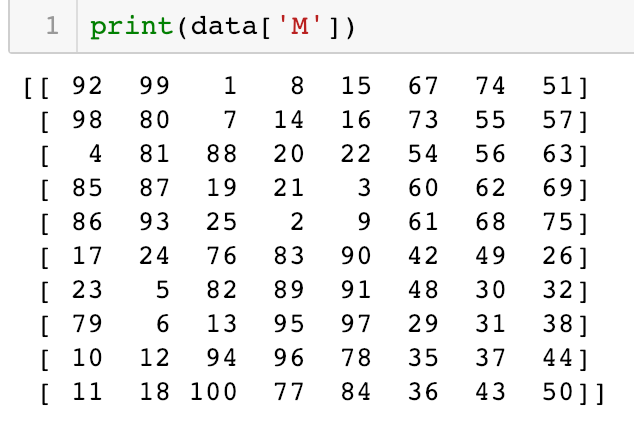
\includegraphics[scale=0.6]{1.png}

\item[ii]
Dimensions of M: (10, 8)\\

\item[iii]
The 4-th row: [85 87 19 21  3 60 62 69]\\
The 5-th column: [15 16 22  3  9 90 91 97 78 84]\\

\item[iv]
the mean value of the 5th column of M: 50.5

\item[v]
The histogram of the 4th row of M is:\\
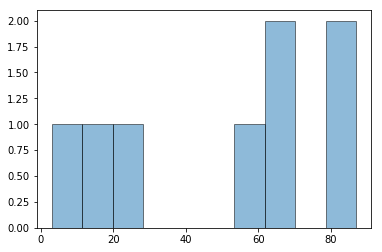
\includegraphics[scale=0.6]{2.png}

\item[vi]
The top three eigenvalues of the matrix $M^TM$ are: 1022.06770617, 263.62801936, 102.8303462\\
\end{enumerate}




\section*{4.2}
\begin{enumerate}
\item[iv]
$\lambda_{max} = 5.52617159, \lambda(min) = 0.72382841$\\

\item[vi]
A histogram of values of $\left \| \widetilde{r} \right \|$ \\
$\lambda_{max}$ and $ \lambda_{min} $ are shown in red\\
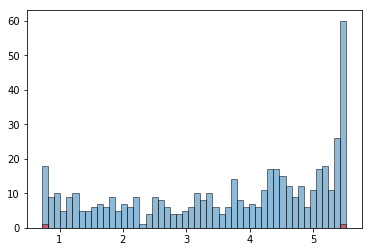
\includegraphics[scale=0.6]{4.png}

\item[vii]
The $\lambda_{max} $ and $\lambda_{min}$ represents the max and min value of the distorted $\left \| \widetilde{r} \right \|$ \\

\item[viii]
vmax = [0.35078, -1]\\

\item[ix]
The histogram is:\\
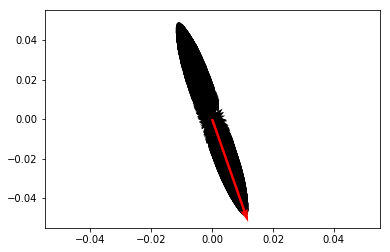
\includegraphics[scale=0.6]{5.png}

\item[x]
vmax points to where changes most, the principle components.

\end{enumerate}


% --------------------------------------------------------------
%     You don't have to mess with anything below this line.
% --------------------------------------------------------------
\end{document}
